\chapter{Fundamentação Teórica}
\label{char:fundteorica}
Inicia-se com uma explicação geral sobre o enquadramento desse trabalho no meio acadêmico com as seções \ref{sec:informaticaeducacao} \nameref{sec:informaticaeducacao} e \ref{sec:objetosaprendizagem} \nameref{sec:objetosaprendizagem}.
 
Na seção \ref{sec:ferramentaspoioensino} \nameref{sec:ferramentaspoioensino}, se dá uma visão geral sobre o que são e qual o ganho que elas trazem para os alunos. A seção, \ref{sec:simuladoresvoltadosensino} \nameref{sec:simuladoresvoltadosensino}, traz uma visão geral sobre simuladores e uma análise de simuladores voltados ao ensino de uma forma geral e a seção \ref{sec:simuladorescriptografia} descreve os simuladores de criptografia atuais.

A seção \ref{sec:criptografia} \nameref{sec:criptografia} discorre sobre criptografia e suas aplicabilidades, assim como seus dois tipos, \ref{subsec:criptografiasync} \nameref{subsec:criptografiasync} e \ref{subsec:criptografiaasync} \nameref{subsec:criptografiaasync}. Apresentam-se suas definições, seus cenários de utilização, e trazem alguns exemplos de algoritmos sobre seus respectivos ramos da criptografia. A seção \ref{sec:cifradeblocos} \nameref{sec:cifradeblocos} fala sobre esse método de criptografia simétrica no qual é feita uma visão geral sobre seu funcionamento e benefícios obtidos por sua utilização.

As seções \ref{sec:des} \nameref{sec:des}, \ref{sec:3des} \nameref{sec:3des} e \ref{sec:sdes} \nameref{sec:sdes} tratam sobre estes algoritmos de criptografia simétrica baseados em cifra de blocos, os quais trazem uma visão geral e uma explicação de cada algoritmo dando uma ênfase maior no \nameref{sec:sdes} por ser o algoritmo utilizado na ferramenta desenvolvida.

\section{Informática na educação}
\label{sec:informaticaeducacao}
A educação abrange dar e receber conhecimento. Qualquer sociedade possui esse cenário, que é responsável pela manutenção e propagação às gerações que se seguem, da cultura necessária à convivência de um membro na sua sociedade \cite{hamawaki09}.

Dentre as formas de aprendizagem, são citadas duas teorias importantes por Ausubel \cite{ausubel80}, a aprendizagem significativa e a mecânica.

A primeira diz respeito à ideia de que a aprendizagem é um processo pelo qual uma informação recém-adquirida relaciona-se com um aspecto importante da estrutura de conhecimento do aluno, ou seja, quando a nova informação adquirida vincula-se em conhecimentos relevantes previamente adquiridos na estrutura cognitiva do aluno. A aprendizagem significativa é onde o aluno realmente aprende.

A aprendizagem mecânica por sua vez ocorre quando o novo conhecimento se associa pouco ou não se associa a algum conhecimento importante já existente na estrutura cognitiva do aprendiz. Quando isso ocorre o conhecimento adquirido recentemente é gravado de maneira arbitrária. Essa aprendizagem é inviável quando um aluno recebe um novo conhecimento em uma área de conhecimentos nova para ele. Ou seja, aprendizagem mecânica acontece somente até que alguns elementos do conhecimento pré-adquirido, relevantes a novas informações na mesma área de conhecimento, existam na estrutura cognitiva do aluno e possam ser utilizadas como base para a aprendizagem significativa. E é através dessa aprendizagem que se inicia a criação, no aluno, de uma estrutura cognitiva mais complexa, onde ele deixa de aprender de forma passiva e mecânica e passa a assimilar o conteúdo de forma mais clara e não linear \cite{ausubel80}.

Muitas vezes a transmissão do conhecimento é árdua e complexa. Tendo em vista essa dificuldade, almeja-se a utilização de bons recursos didáticos que melhorem o desempenho docente. \cite{souza07}. Uma das considerações que devem ser levadas em conta pelo educador como critério de escolha de um recurso didático é que sua utilização deve preencher as lacunas existentes no ensino tradicional e viabilizar ao aluno a ampliação 
tanto da capacidade de reter conhecimento quanto a sua visão, e ainda estimular o ensino docente. \cite{trivelato06}

Sons, imagens, construção de maquetes e até o uso de materiais lúdicos, esses simples elementos podem ser aplicados como recursos didáticos. Quando o corpo docente se utiliza de tipos variados de recursos didáticos ele não somente faz com que o ensino seja mais interessante do que o ensino tradicional, como também pode propiciar melhores resultados \cite{parra85} \cite{souza07} \cite{costoldi09}. Dentre os recursos didáticos que podem ser utilizados existem vários tipos, como: livros, apostilas, artigos, quadro e giz, apresentações, maquetes, trabalhos acadêmicos, softwares, ilustrações, filmes, músicas, exercícios físicos, excursões, brincadeiras e outros \cite{ferreira07}. A brincadeira Adedonha, por exemplo, já teve sua eficiência comprovada como ferramenta prático-pedagógica no processo de ensino-aprendizagem \cite{silva18}.

A abordagem do uso do computador e/ou dispositivos eletrônicos similares como recurso pedagógico utilizado pelo docente no processo de ensino do corpo discente é conhecido como Informática na educação. \cite{kenski07}

\section{Objetos de aprendizagem}
\label{sec:objetosaprendizagem}

\textit{"...definimos objetos de aprendizagem como sendo recursos digitais dinâmicos, interativos e reutilizáveis em diferentes ambientes de aprendizagem elaborados a partir de uma base tecnológica. Desenvolvidos com fins educacionais, eles cobrem diversas modalidades de ensino: presencial, híbrida ou à distância; diversos campos de atuação: educação formal, corporativa ou informal; e, devem reunir várias características como durabilidade, facilidade para atualização, flexibilidade, interoperabilidade, modularidade, portabilidade, entre outras. Eles ainda apresentam-se como unidades autoconsistentes de pequena extensão e fácil manipulação, passíveis de combinação (essa combinação dá-se, principalmente, no sentido objeto-mídia, mas o contrário também é válido dependendo da mídia, pois não são todas que oferecem a característica de hiperligação) com outros objetos educacionais ou qualquer outra mídia digital (vídeos, imagens, áudios, textos, gráficos, tabelas, tutoriais, aplicações, mapas, jogos educacionais, animações, infográficos, páginas web) por meio da hiperligação. Além disso, um objeto de aprendizagem pode ter usos variados, seu conteúdo pode ser alterado ou reagregado, e ainda ter sua interface e seu layout modificado para ser adaptado a outros módulos ou cursos. No âmbito técnico, eles são estruturas autocontidas em sua grande maioria, mas também contidas, e marcadas por identificadores denominados metadados."} \cite{audino12}

Em suma, um \acrfull{oa} é um recurso digital utilizado para suportar o ensino. Imagens, vídeos, softwares e animações podem ser considerados \acrshort{oa}s contanto que sejam voltados ao ensino. Já os \acrfull{avas} por sua vez não são considerados \acrshort{oa}s pois esses, apesar de gerenciar e até armazenar \acrshort{oa}s, não são utilizados diretamente na aprendizagem. \cite{wiley02} \cite{braga14}

Apesar do AVA ser o principal instrumento mediador em um sistema de \acrfull{ead} isso não exclui sua utilização como suporte para o ensino presencial \cite{belmonte10}.

\section{Ferramentas de apoio ao ensino}
\label{sec:ferramentaspoioensino}

Ainda é um desafio a criação de \acrshort{oa}s pois geralmente o conhecimento pedagógico é detido por um profissional da área de ensino e este normalmente não possui o conhecimento técnico avançando necessário para o desenvolvimento de \acrshort{oa}s \cite{braga15}.

Há também \acrshort{oa}s que podem ser customizadas e aplicadas para várias áreas de ensino, como é o caso do jogo \textit{Minecraft: Education Edition} que já foi aplicado no ensino de Biologia, Ecologia, Física, Química, Geologia, Geografia \cite{short12} e até Cibersegurança \cite{geary19}, .

Existe um problema comum entre professores e alunos de disciplinas do curso de Ciência da Computação: Existe uma dificuldade em demonstrar a real dinâmica dos eventos computacionais. Mesmo que o mestre tenha conhecimento e didática, que o aluno dedique raciocínio e atenção, nem sempre é possível se obter a total compreensão dos conceitos ensinados diante da abordagem destes nas disciplinas.

O computador não deve ser o substituto do professor, mas sim, tomar o papel de ferramenta educacional auxiliando o aprendizado. Com isso o papel do professor passa a ser mais produtivo. Primeiramente, ferramentas voltadas ao ensino, já se utilizando do computador, se baseavam na máquina de \textit{B. F. Skinner}, onde se utilizava a ideia de instrução programada, que consistia de dividir o conteúdo total em pequenas partes lógicas e sequenciais. Somente durante a década de 1960, foi dado inicio ao conceito de \acrfull{cai}, ou seja, \acrfull{pec}. A real dispersão do \acrshort{cai} só aconteceu com popularização dos microcomputadores, possibilitando assim, a criação de diversos tipos de ferramentas de ensino, como, tutoriais, exercício-e-prática, avaliações, jogos, e simulações \cite{hamawaki09}.

\section{Simuladores voltados ao ensino}
\label{sec:simuladoresvoltadosensino}

Algumas situações são tão singulares, que se preparar para tais torna-se difícil. E portanto, com o intuito de proporcionar a alguém um conhecimento maior sobre estas situações os simuladores foram criados.

A simulação é uma representação do mundo real. As primeiras simulações foram criadas com o intuito de disponibilizar um ambiente seguro para situações que envolvessem risco ao humano. Dentre elas podemos citar simulações de viagens e mergulhos profundos. Posteriormente, foram criadas com o intuito de se obter uma economia, seja ela de tempo e/ou dinheiro, que é o caso da indústria automobilística e aviação.

Diversas são as áreas de conhecimento que fazem uso das simulações \cite{banks09}. Na ciência da computação há uma disponibilidade de simuladores, cada um atendendo a uma respectiva disciplina, assim como redes de computadores, arquitetura de computadores, técnicas de programação e sistemas operacionais.

Os simuladores possuem um potencial bem maior do que as outras ferramentas de ensino citadas acima. A aplicação de simulações no universo acadêmico permite que o aluno desenvolva hipóteses, teste-as, analise os resultados e concretize seus conhecimentos. Simuladores devem ser utilizados como ferramenta complementar as aulas lecionadas pelo professor.

Mesmo com todas as vantagens envolvidas, o desenvolvimento de um simulador não é algo trivial. Uma vez que a ferramenta possui um cunho pedagógico, a utilização de recursos multimídia para tornar a simulação mais fiel à realidade é muito importante, e a utilização destes recursos não é algo de simples desenvolvimento.

Quando o aluno possui pouco conhecimento na área, os simuladores são indicados como melhor ferramenta de auxilio. Principalmente, se forem para auxiliar cursos de extensão e graduação \cite{maia01} \cite{maia03}. 

\section{Simuladores de criptografia}
\label{sec:simuladorescriptografia}
Essa seção descreve alguns simuladores de criptografia.

Além dos simuladores descritos nas seções seguintes foram encontrados o "Crypto-tutor: \textit{An educational tool for learning modern cryptography}" \cite{luburic16} e o CET - \textit{Cryptographic Education Tool} \cite{abuzaid11}. Porém um estudo sobre estes não pôde ser feito pois os simuladores não estão disponíveis para uso e suas publicações científicas não estão disponíveis publicamente.

\subsection{CyberChef}

\begin{figure}[H]
    \centering
    \caption{Simulador: CyberChef}
    \label{fig:cyberchef}
    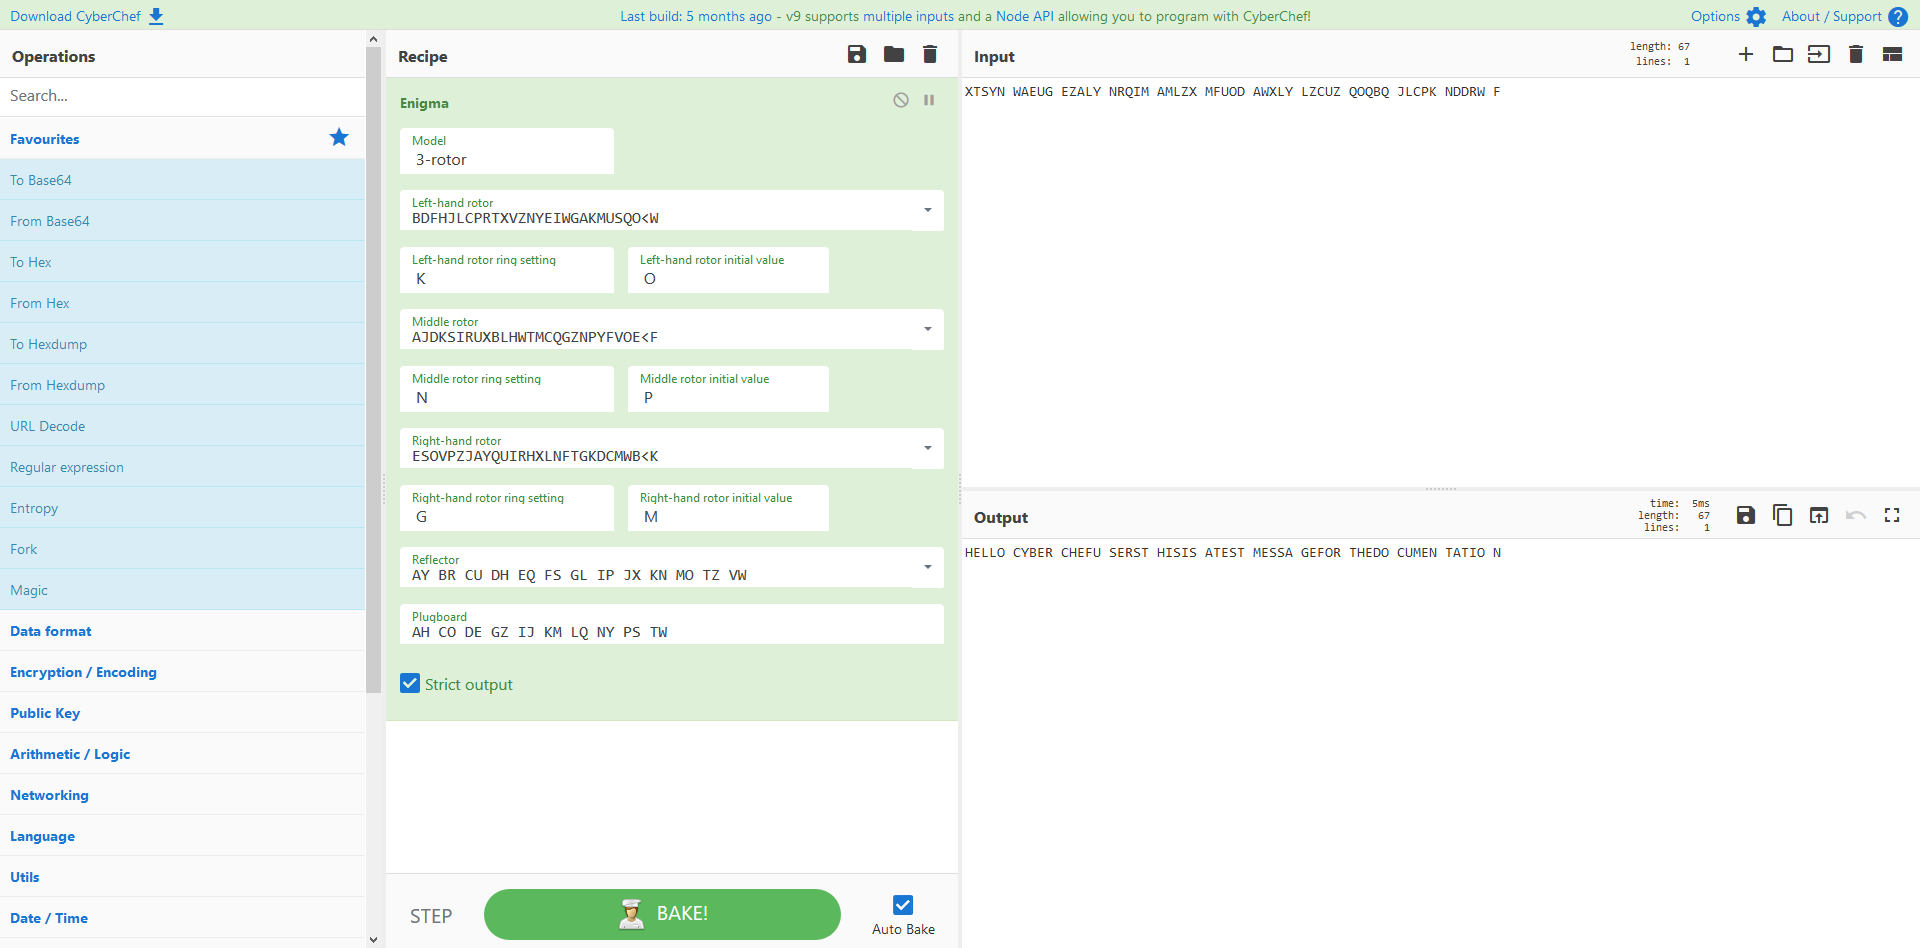
\includegraphics[width=1.2\linewidth,center]{Simuladores/CyberChef_Enigma.png}
    \legend{Fonte: \cite{gchq20}}
\end{figure}

O CyberChef (Figura \ref{fig:cyberchef}) trata-se de um simulador da máquina enigma criado pela \acrfull{gchq}, o centro de inteligência britânica. Ele está disponibilizado no idioma inglês e permite a utilização de vários algoritmos simples (como \textit{ToBase64String} e etc.), podendo inclusive encadear a execução destes sobre o \textit{input}. Nele pode-se informar os parâmetros de entrada que ele utiliza para mostrar o resultado da execução do algoritmo. Ele não é voltado ao ensino e sim para testes dos algoritmos com entradas customizadas. Ele possui o código aberto e este está disponibilizado em \textit{https://github.com/gchq/CyberChef/}. O simulador pode ser utilizado em \textit{browsers} pois está \textit{online} no endereço \textit{https://gchq.github.io/CyberChef/}. \cite{gchq20}

%\begin{itemize}
    %\item Disponibilizado \textit{online} em \textit{https://gchq.github.io/CyberChef/}.
    %\item Idioma: Inglês.
    %\item Possui vários algoritmos simples.
    %\item Mostra somente entradas e saídas.
    %\item Possui atualmente vários algoritmos.
    %\item Pode encadear criptografias que serão aplicadas sequencialmente sobre o \textit{input}.
    %\item Não é direcionado ao ensino.
    %\item Disponibilizado no \textit{GitHub} (\textit{https://github.com/gchq/CyberChef/}).
%\end{itemize}

\subsection{CrypTool}

\textit{CrypTool} é um portal de criptografia (\textit{https://www.cryptool.org/en/}) que disponibiliza alguns simuladores de criptografia. Ele foi criado pela contribuição de várias instituições de vários locais do mundo, por exemplo: \textit{University of Siegen} (Germany), \textit{Politechnika Warszawska} (Poland), \textit{Consejo Superior de Investigaciones Científicas} (Spain), \textit{Klagenfurt University} (Austria) e \textit{University of Singidunum} (Serbia). \cite{cryptool20}

\subsubsection{CrypTool 2}

\begin{figure}[H]
    \centering
    \caption{Simulador: CrypTool 2}
    \label{fig:cryptool2}
    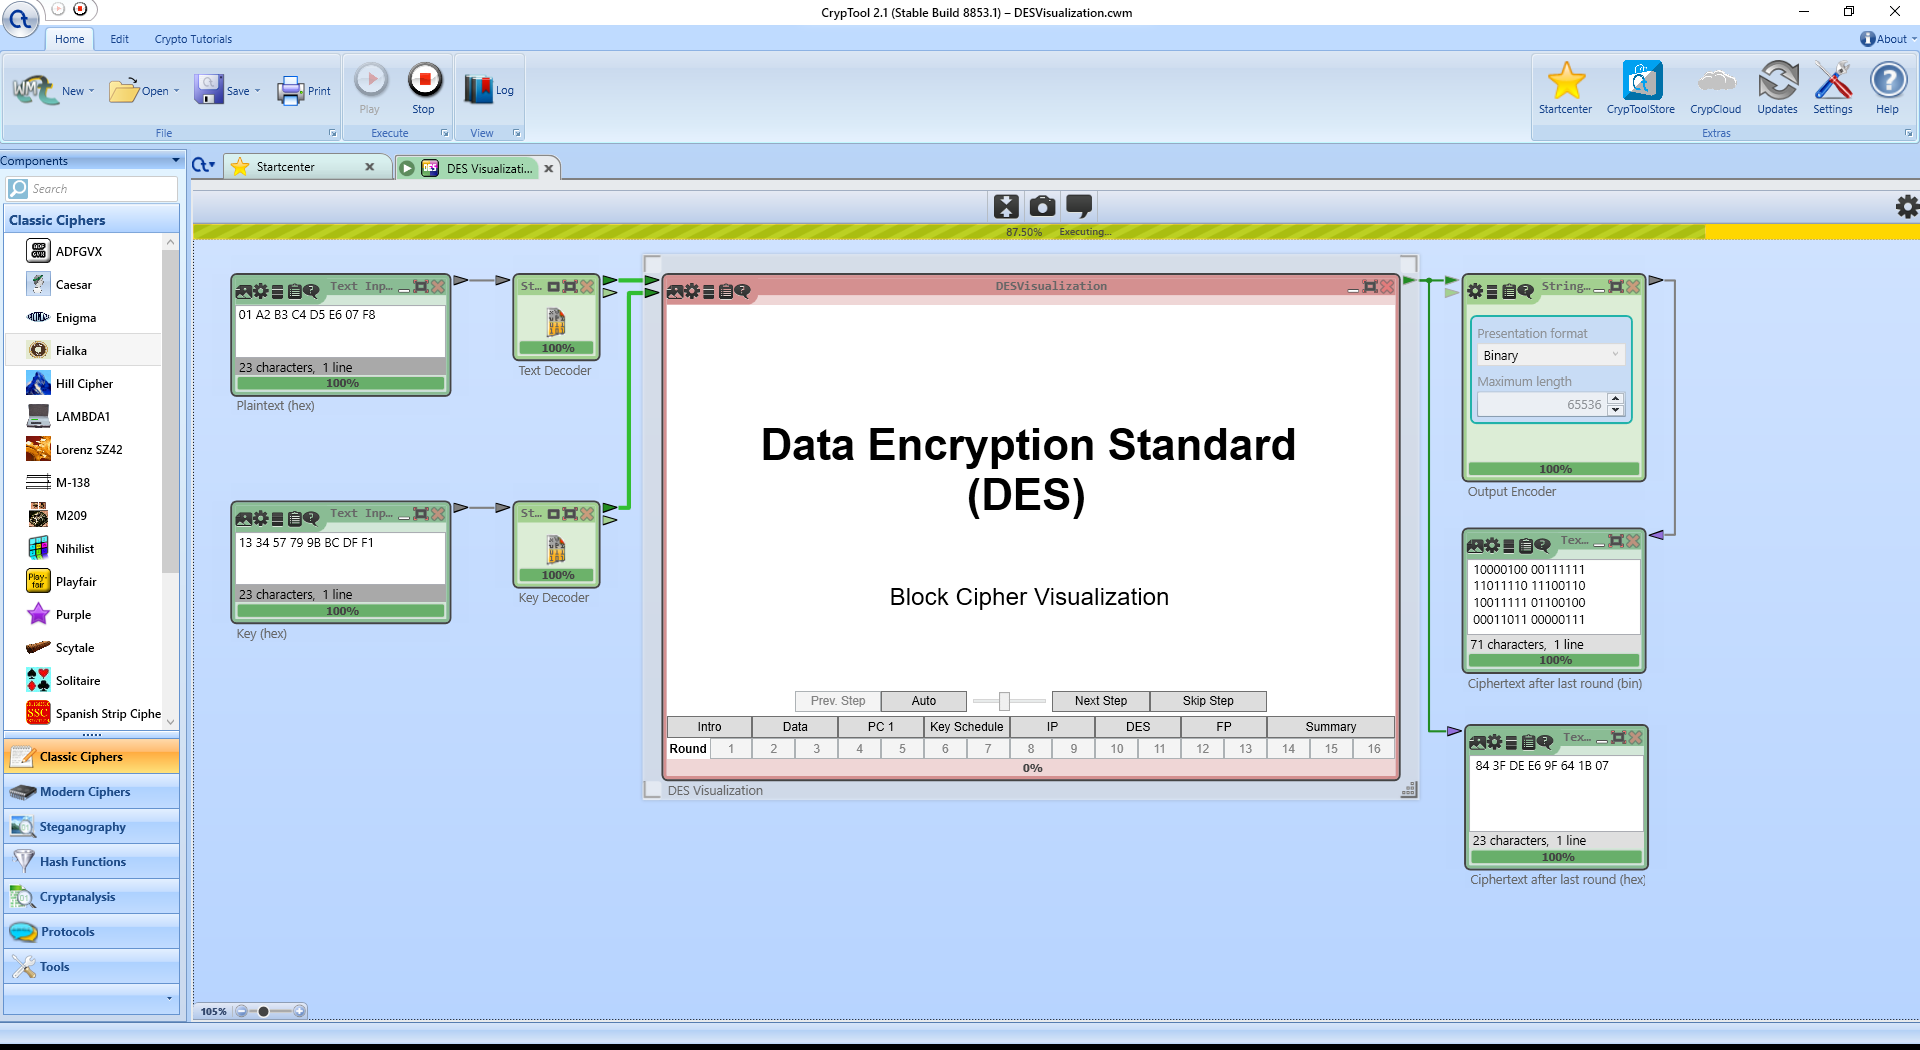
\includegraphics[width=1.2\linewidth,center]{Simuladores/CrypTool2.png}
    \legend{Fonte: do autor}
\end{figure}

O CrypTool 2 (Figura \ref{fig:cryptool2}) está disponibilizado no idioma inglês e permite a utilização de vários algoritmos através da disponibilização de \textit{templates} que podem ser criados pelos colaboradores. Nele pode-se informar os parâmetros de entrada que ele utiliza para mostrar o fluxo e resultado da execução do algoritmo. Ele é voltado ao ensino e também para testes dos algoritmos com entradas customizadas, dependendo do \textit{template} escolhido. Só foi encontrado 1 \textit{template} voltado ao ensino (a existência de \textit{templates} voltados ao ensino dependem dos contribuidores). Ele possui o código aberto e este está disponibilizado em \textit{https://www.cryptool.org/en/}. O simulador pode ser instalado somente no Windows e apresenta uma interface complexa e com muitas interações possíveis visíveis simultaneamente. \cite{cryptool14}

%\begin{itemize}
    %\item Só pode ser instalado em Windows.
    %\item Idioma: Inglês.
    %\item Tem um conjunto de \textit{templates} de algoritmos expansível.
    %\item Possui somente 1 \textit{template} que executa passo a passo.
    %\item Interface complexa e de difícil utilização.
    %\item É direcionado ao ensino.
%\end{itemize}

\subsubsection{JCrypTool}

\begin{figure}[H]
    \centering
    \caption{Simulador: JCrypTool}
    \label{fig:jcryptool}
    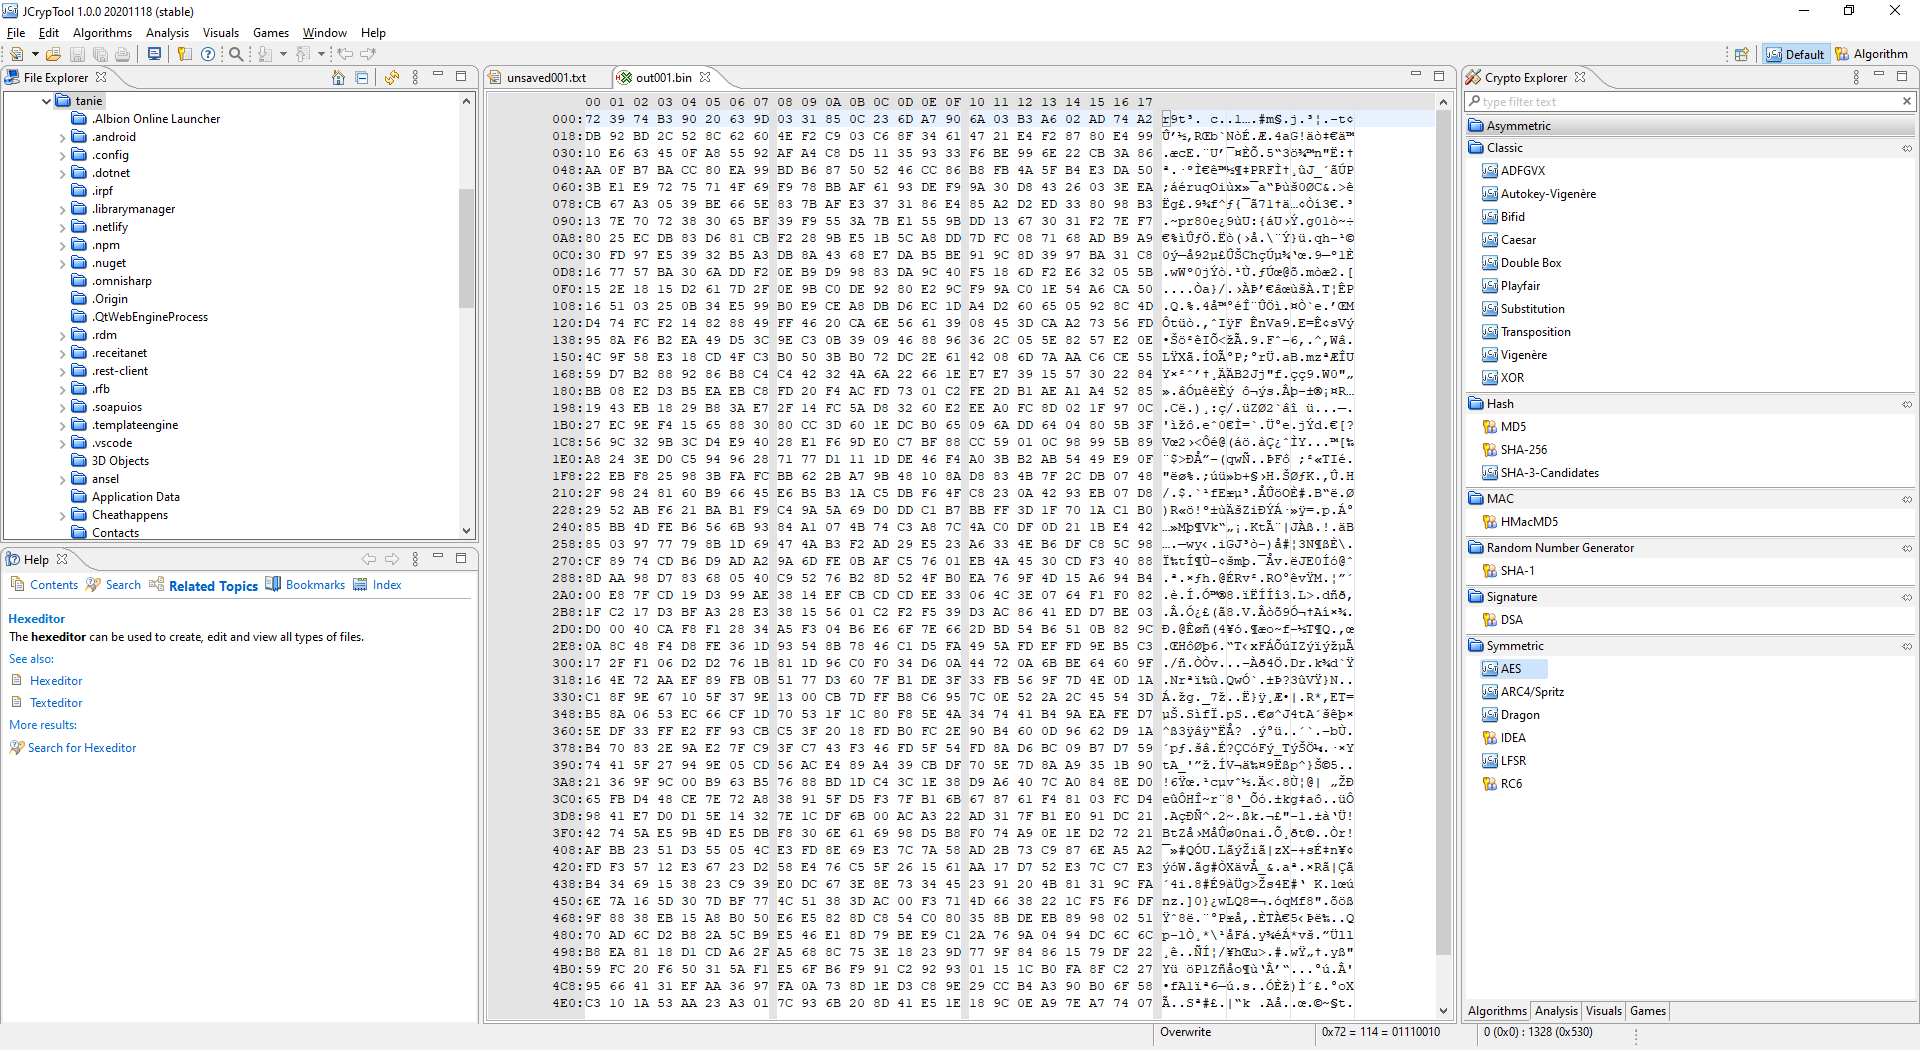
\includegraphics[width=1.2\linewidth,center]{Simuladores/JCrypTool.png}
    \legend{Fonte: do autor}
\end{figure}

O JCrypTool (Figura \ref{fig:jcryptool}) está disponibilizado no idioma inglês, foi feito em java se utilizando como base a interface do \textit{Eclipse} e permite a utilização de vários algoritmos através da disponibilização de \textit{templates} que podem ser criados pelos colaboradores. Nele pode-se informar os parâmetros de entrada que ele utiliza para mostrar o resultado da execução do algoritmo. Ele é voltado ao ensino e para testes dos algoritmos com entradas customizadas, dependendo do \textit{template} escolhido. Não foi encontrado \textit{template} voltado ao ensino (a existência de \textit{templates} voltados ao ensino dependem dos contribuidores). Ele possui o código aberto e este está disponibilizado em \textit{https://www.cryptool.org/en/}. O simulador pode ser instalado em versões mais recentes do Windows, Linux e macOS e apresenta uma interface complexa e com muitas interações possíveis visíveis simultaneamente. \cite{cryptool16}

%\begin{itemize}
    %\item Desenvolvida em Java e pode ser instalado em Linux, Mac and Windows.
    %\item Idioma: Inglês.
    %\item Tem um conjunto de \textit{templates} de algoritmos expansível.
    %\item Não possui \textit{template} que executa passo a passo.
    %\item Interface complexa e de difícil utilização.
    %\item É direcionado ao ensino.
%\end{itemize}

\subsection{S-DES Simulator (\textit{Android App})}

\begin{figure}[H]
    \centering
    \caption{Simulador: S-DES Simulator}
    \label{fig:sdessimulatorapp}
    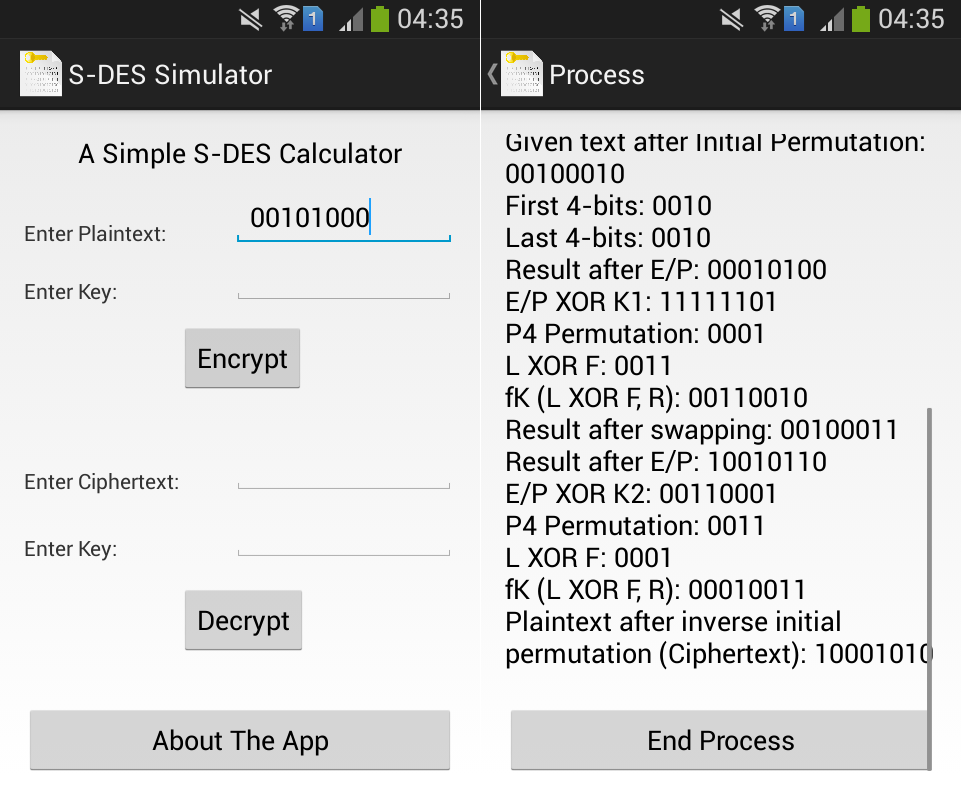
\includegraphics[width=.75\linewidth]{Simuladores/SDESSimulatorApp.png}
    \legend{Fonte: do autor}
\end{figure}

O S-DES Simulator (Figura \ref{fig:sdessimulatorapp}) está disponibilizado no idioma inglês e permite a execução do S-DES, incluindo os resultados obtidos em cada passo. Nele pode-se informar os parâmetros de entrada que ele utiliza para mostrar os resultados dos passos e o resultado da execução do algoritmo. Ele é voltado ao ensino. O simulador foi desenvolvido para uma versão bem antiga do Android então precisa ser habilitado modo de compatibilidade na \textit{App Store} e mesmo depois de instalado um aviso sempre aparece ao iniciar o aplicativo como mostra a figura \ref{fig:sdessimulatorappwarning}. \cite{mountogiannakis15}

\begin{figure}[H]
    \centering
    \caption{Simulador: S-DES Simulator's warning}
    \label{fig:sdessimulatorappwarning}
    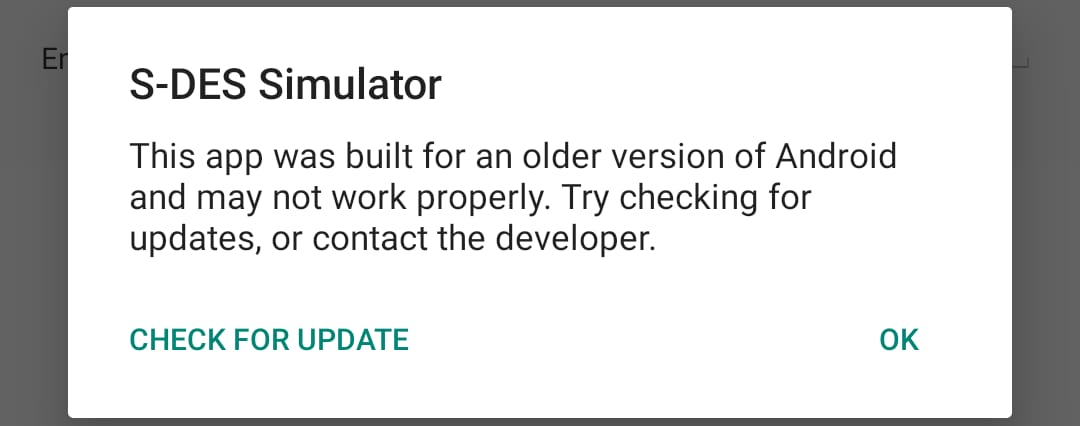
\includegraphics[width=.55\linewidth]{Simuladores/SDESSimulatorAppWarning.jpeg}
    \legend{Fonte: do autor}
\end{figure}

%\begin{itemize}
    %\item Pode ser instalado em versões antigas do \textit{Android}. Foi necessário usar um simulador para poder testar.
    %\item Idioma: Inglês.
    %\item Só possui o \acrshort{sdes} como possível algoritmo.
    %\item Executa passo a passo mas só mostra os resultados dos passos.
    %\item É direcionado ao ensino.
%\end{itemize}

\subsection{S-DES Simulator (\textit{online})}

\begin{figure}[H]
    \centering
    \caption{Simulador: S-DES Simulator}
    \label{fig:sdessimulatorkr}
    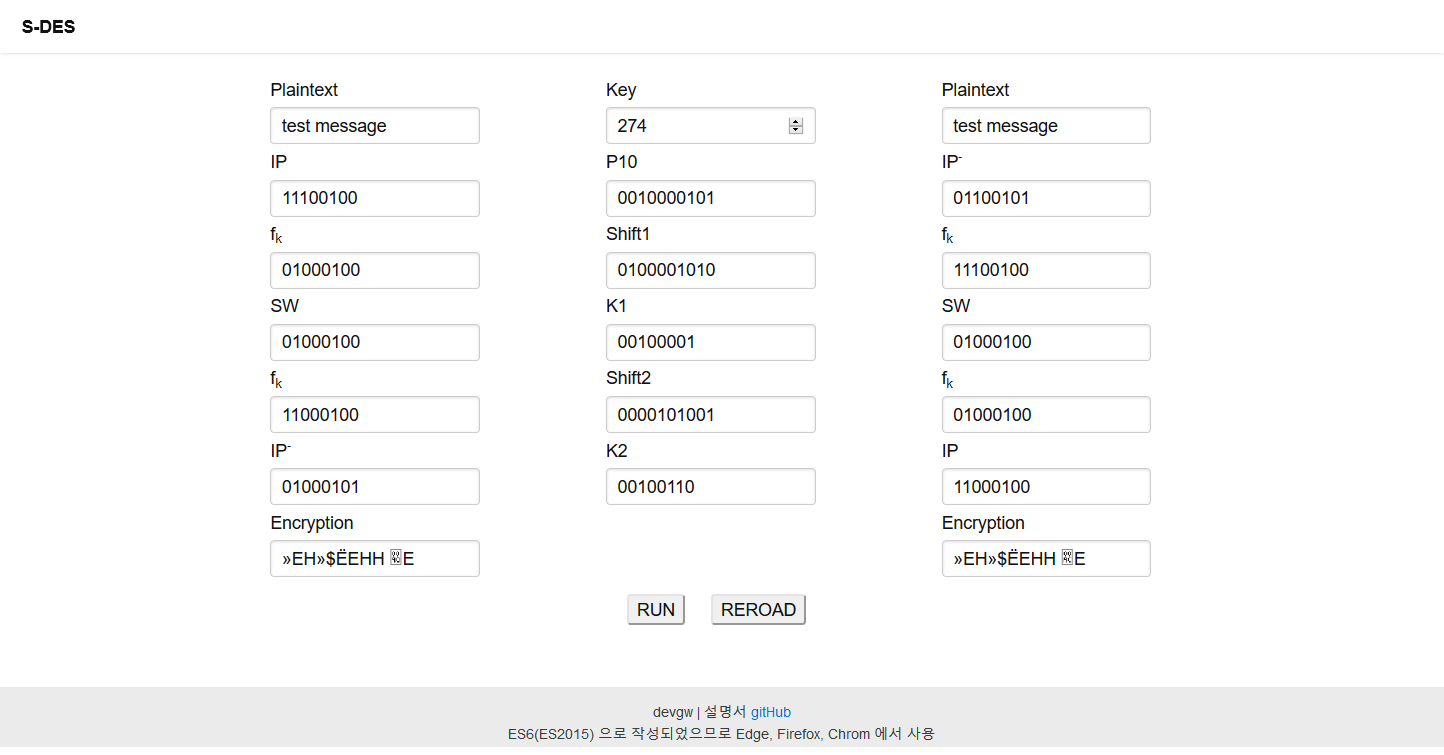
\includegraphics[width=1.2\linewidth,center]{Simuladores/SDESSimulatorKr.png}
    \legend{Fonte: do autor}
\end{figure}

O S-DES Simulator (Figura \ref{fig:sdessimulatorkr}) está disponibilizado no idioma koreano e permite a execução do S-DES, incluindo os resultados obtidos em cada passo. Nele pode-se informar os parâmetros de entrada que ele utiliza para mostrar os resultados dos passos e o resultado da execução do algoritmo. Ele é voltado ao ensino. Ele possui o código aberto e este está disponibilizado em \textit{https://github.com/devGW/S-DES-simulator/}. O simulador pode ser utilizado em \textit{browsers} pois está \textit{online} no endereço \textit{https://devgw.github.io/S-DES-simulator/}. \cite{woo18}

%\begin{itemize}
    %\item Disponibilizado \textit{online} em \textit{https://devgw.github.io/S-DES-simulator/}.
    %\item Idioma: Koreano.
    %\item Só possui o \acrshort{sdes} como possível algoritmo.
    %\item Executa passo a passo mas só mostra os resultados dos passos.
    %\item É direcionado ao ensino.
    %\item Disponibilizado no \textit{GitHub} (\textit{https://github.com/devGW/S-DES-simulator}).
%\end{itemize}

\subsection{S-DES Simulator (Win)}

\begin{figure}[H]
    \centering
    \caption{Simulador: S-DES Simulator}
    \label{fig:sdessimulatoren}
    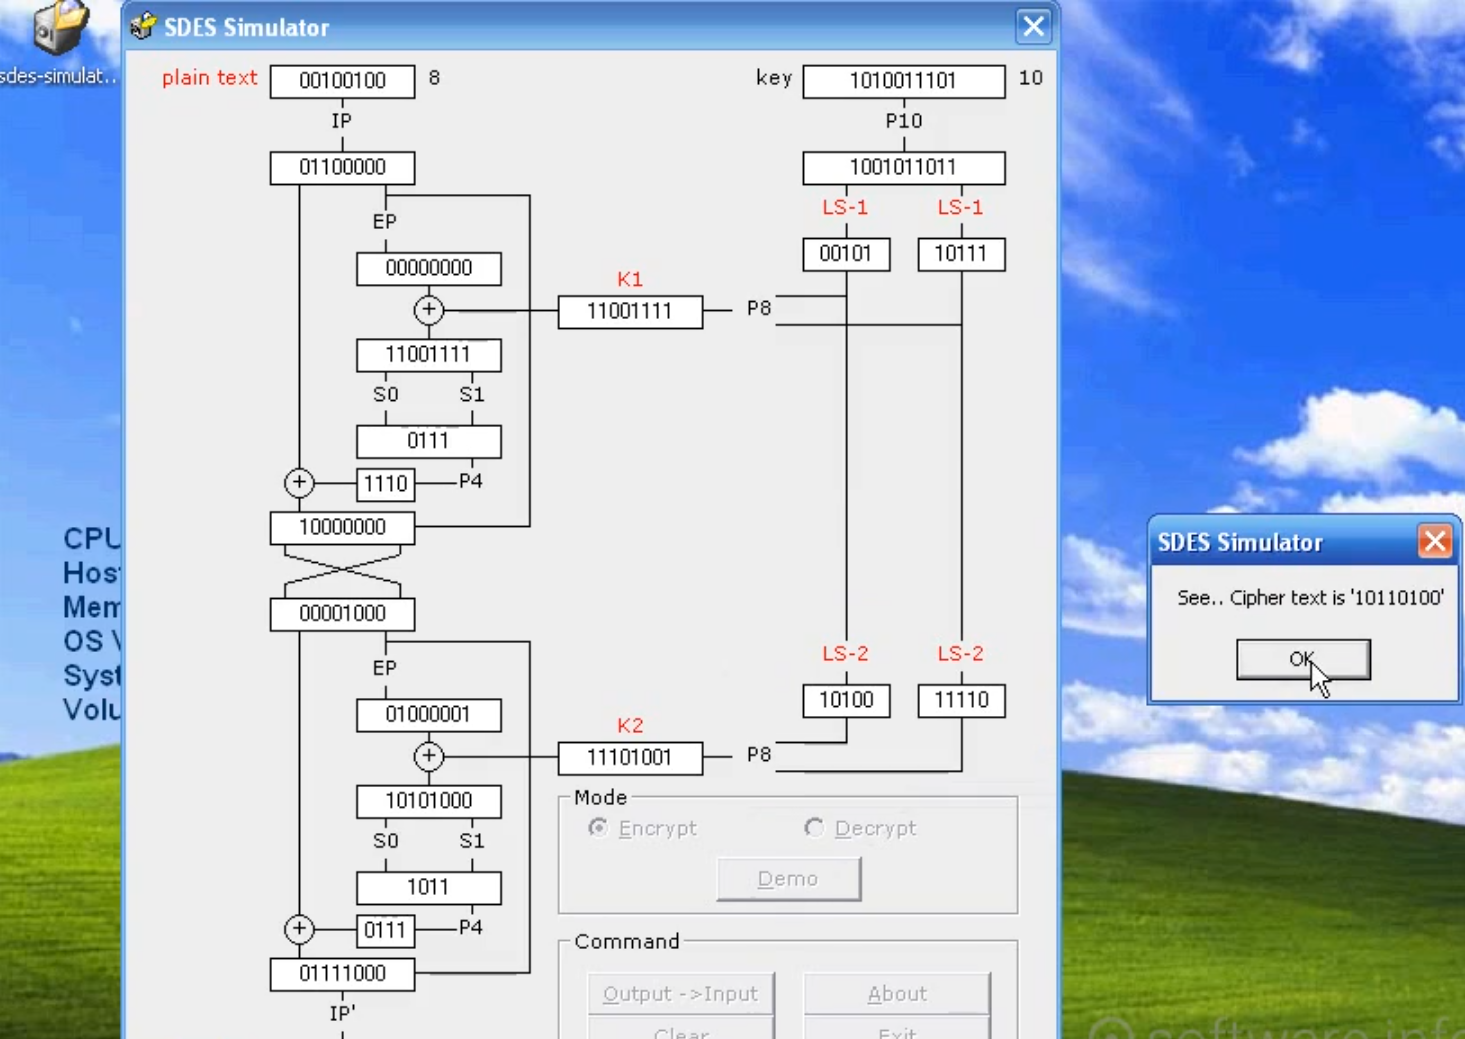
\includegraphics[width=1.2\linewidth,center]{Simuladores/SDESSimulatorXp.png}
    \legend{Fonte: do autor}
\end{figure}

O S-DES Simulator (Figura \ref{fig:sdessimulatoren}) está disponibilizado no idioma inglês e permite a execução do S-DES, incluindo os resultados obtidos em cada passo. Nele pode-se informar os parâmetros de entrada que ele utiliza para mostrar os resultados dos passos e o resultado da execução do algoritmo. Ele é voltado ao ensino e pode ser instalado no Windows. \cite{permadi18}

%\begin{itemize}
    %\item Só pode ser instalado em Windows.
    %\item Idioma: Inglês.
    %\item Só possui o \acrshort{sdes} como possível algoritmo.
    %\item Executa passo a passo mas só mostra os resultados dos passos.
    %\item É direcionado ao ensino.
%\end{itemize}

%\section{História}
%\label{sec:historia}
%Há algumas décadas atrás, antes que se fosse comum o uso de equipamentos de processamento de dados, a segurança da informação que era considerada importante para uma empresa se dava basicamente através de dois meios: o administrativo e o físico. Um bom exemplo para o meio administrativo é o uso de um processo de aquisição de profissionais bastante seleto e rigoroso, assim como a utilização de um contrato de confidencialidade que protege a empresa de possíveis ‘vazamentos’ de dados. Um bom exemplo para o meio físico é o uso de cofres e senhas para armazenar documentos importantes ou até confidenciais.

%Com o surgimento do computador surgiu a necessidade de proteger virtualmente os arquivos, agora armazenados de forma virtual no computador. Essa necessidade é ainda mais evidente com o surgimento da Internet, que traz uma facilidade de comunicação muito grande entre os computadores.

%O \acrfull{iab} emitiu, em 1994, um relatório de título “Security in the internet architecture” (Segurança na arquitetura da Internet). O documento estabelecia que a internet necessitava de mais e melhor segurança. Entre as principais áreas citadas no relatório como sendo as que mais necessitavam de segurança estavam a infraestrutura da rede contra monitoração e controle não autorizados do tráfego da rede e também a necessidade de proteger o tráfego entre usuários finais se utilizando de autenticações e criptografias.

%Com o passar dos anos, os ataques através da Internet se tornaram mais evoluídos, eles se tornaram mais automatizados e mais devastadores, necessitando cada vez mais de formas de segurança também mais evoluídas \cite{stallings14}.

%Existe uma lista de mecanismos de segurança explicitados na recomendação X.800 \cite{itu91}. Entre eles temos a cifragem, que é melhor descrita mais adiante. A X.800 divide, muito claramente, dois tipos de criptografia, a reversível e a irreversível. A criptografia reversível é composta por um algoritmo matemático que permite que dados sejam criptografados e que estes dados criptografados possam ser decriptografados posteriormente. Já a criptografia irreversível, por sua vez, é capaz de criptografar os dados, mas a decriptografia desses dados é impossível. Esta por sua vez tem objetivos diferentes da reversível, que visa somente trafegar ou armazenar dados de maneira segura, ela é composta de algoritmos de hash e tem como objetivo autenticação e assinatura digital \cite{stallings14} \cite{itu91}.

\section{Criptografia}
\label{sec:criptografia}
Segundo a National Research Council (1991, apud STALLINGS, 2008, pg. 15), “A criptografia provavelmente é o aspecto mais importante da segurança de comunicações e está se tornando cada vez mais importante como um componente básico para a segurança do computador.”.

O termo Criptografia vem do Grego \textit{kryptós}, que significa “escondido” e de \textit{gráphein}, que significa “escrita”. Ela é o estudo dos princípios e técnicas pelas quais os dados podem ser transformados da sua forma original em outra ilegível. Dessa forma, os dados podem ser conhecidos somente pelo destinatário, o detentor da “chave secreta”, o que faz com que mesmo que tenham sido interceptados, torne difícil a leitura de seu conteúdo por alguém não autorizado. Ela faz parte da Criptologia e é um sub-ramo da Matemática \cite{knudsen98}.

O estudo da maneira de camuflar o real significado de uma mensagem usando técnicas e algoritmos de cifragem têm evoluído juntamente com o estudo da maneira de se conseguir entender a mensagem quando não se é o real destinatário da mesma. Este campo de estudo é chamado Criptoanálise \cite{gaines56}. A Criptologia engloba a Criptografia e a Criptoanálise. Alguns autores se utilizam do termo Criptovirologia quando falam de vírus que se utilizam de chaves publicas \cite{young04}.

%Há também a Esteganografia que não faz parte de Criptologia, mesmo sendo estudada em situações bem similares e até pelos mesmos autores. Ao contrário da criptografia que modifica a informação com intuito de transformar seu estado original em algo indecifrável a Esteganografia estuda formas de como se pode camuflar uma informação dentro de outra. Temos também a Esteganálise que está para Esteganografia assim como a Criptoanálise está para a Criptografia \cite{salomon05}.

A criptografia se divide em Simétrica, também chamada de criptografia convencional, e Assimétrica, também chamada de criptografia por chave pública \cite{stallings14} \cite{tanenbaum03} e dentro dessa divisão ainda temos algoritmos de criptografia reversíveis e irreversíveis \cite{stallings14} \cite{itu91}.

A criptografia possui inúmeras áreas de aplicação. Desde transações bancárias, envio de e-mails, segurança de arquivos sigilosos, segurança de autenticação, armazenamento de senhas em bancos de dados até o sinal de linha telefônica, sinal de TV digital e acesso a sites certificados \cite{avelino07}.

\subsection{Criptografia Simétrica}
\label{subsec:criptografiasync}
Também chamada de criptografia convencional, a criptografia simétrica é um criptosistema no qual tanto a criptografia como a decriptografia são realizadas com a mesma chave.

Ela transforma uma mensagem clara em uma mensagem cifrada, usando um algoritmo de criptografia e uma chave. Esta mesma chave juntamente com a inversão do algoritmo utilizado (gerando assim o algoritmo de decriptografia do algoritmo), são necessários para que se possa obter a mensagem clara novamente a partir da mensagem cifrada, assim como demonstra a Figura \ref{fig:cripsimerica}.

\begin{figure}[H]
    \centering
    \caption{Criptografia Simétrica}
    \label{fig:cripsimerica}
    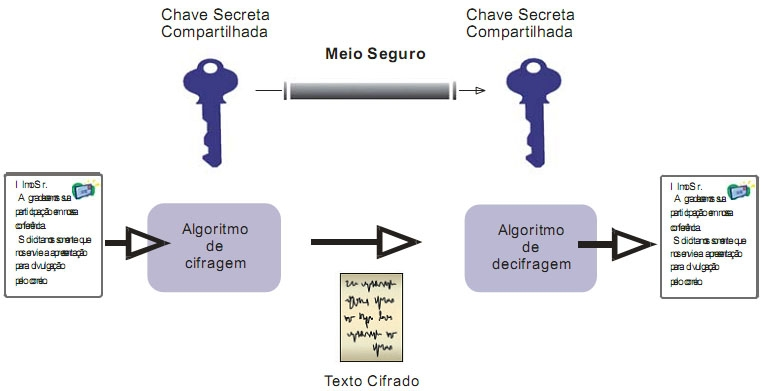
\includegraphics[width=.8\linewidth]{Figuras/CripSimetrica.jpg}
    \legend{Fonte: \cite{brocardo06}}
\end{figure}

Antes do computador, as cifras simétricas tradicionais poderiam se utilizar de técnicas de transposição ou de substituição, ou até as duas técnicas combinadas. Essas técnicas são os componentes básicos para todas as técnicas de criptografia.

Técnicas de transposição transpõem sistematicamente as posições dos elementos da mensagem clara. Tal técnica consiste na aplicação de alguma permutação na mensagem clara de forma que a mensagem final seja ilegível, e somente o detentor da forma de como os elementos da mensagem foram permutados pode obter novamente a mensagem de forma clara. A cifra mais simples dessa técnica é a cifra de \textit{Rail fence}. A Figura \ref{fig:railfence} ilustra como ficaria a crifa \textit{Rail fence} de profundidade dois do texto “Técnica de transposição”.

\begin{figure}[H]
    \centering
    \caption{Exemplo de \textit{Rail fence}}
    \label{fig:railfence}
    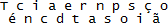
\includegraphics{Figuras/RailFence.png}
    \legend{Fonte: do autor}
\end{figure}

Técnicas de substituição mapeiam elementos, caracteres ou bits, da mensagem clara e as substitui por outras letras ou números ou até símbolos. Analisando a mensagem clara como sendo um conjunto de bits, então a substituição é definida pela troca de padrões de bits da mensagem clara por padrões de bits da mensagem cifrada. Como exemplo clássico temos a cifra de César, criada por Júlio César. A Figura \ref{fig:cifradecesar} ilustra como ficaria a cifra de César com o texto “Tecnica de substituicao”.

\begin{figure}[H]
    \centering
    \caption{Exemplo de cifra de César}
    \label{fig:cifradecesar}
    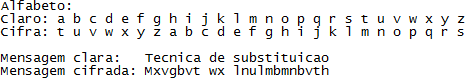
\includegraphics{Figuras/CifraDeCesar.png}
    \legend{Fonte: do autor}
\end{figure}

Existem basicamente dois os ataques possíveis em um algoritmo criptográfico. A criptoanálise, que se baseia nas características do próprio algoritmo de criptografia, e a força bruta, que engloba simplesmente repetidas tentativas de todas as chaves possíveis até encontrar a correta.

Antes da existência do computador existiam máquinas que implementavam a nível de hardware técnicas de substituição. Eram conhecidas como máquinas de rotor. Duas foram as máquinas de rotor mais conhecidas, a da Alemanha, conhecida como Enigma e a do Japão conhecida como Purple. Elas foram utilizadas durante a segunda guerra mundial e a quebra desses dois códigos pelos Aliados foi significante para o resultado da guerra. Abaixo, a Figura \ref{fig:maqenigma} mostra a máquina Enigma com três rotores.

\begin{figure}[H]
    \centering
    \caption{Imagem da máquina Enigma}
    \label{fig:maqenigma}
    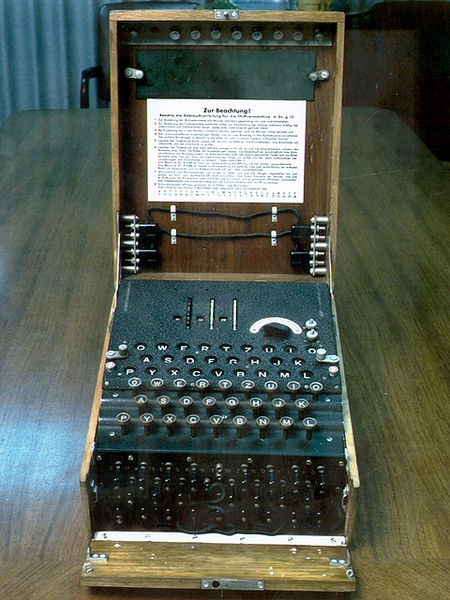
\includegraphics[width=.35\linewidth]{Figuras/MaqEnigma.jpg}
    \legend{Máquina Enigma com três rotores, teclado, luzes e conexões para câmbio de codificação. Fonte: Wikipedia. Fonte: \cite{maqenigma20}}
\end{figure}

Algoritmos simétricos são utilizados em cenários em que a mensagem tem uma necessidade de ser decriptografada, por exemplo, o Kerberos, serviço de autenticação desenvolvido no \textit{Massachusetts Institute of Technology} (MIT) como parte do projeto Athena, que visa trazer segurança a cenários distribuídos abertos, se utiliza unicamente de cifra simétrica \cite{stallings14} \cite{tanenbaum03}.

\subsection{Criptografia Assimétrica}
\label{subsec:criptografiaasync}
Também chamada de criptografia por chave pública, a criptografia assimétrica é um criptosistema onde a criptografia e a decriptografia são realizadas com chaves diferentes, uma pública e outra privada. Quando uma mensagem é criptografada com uma chave, somente a outra chave poderá decriptografar  a mensagem. O criptosistema assimétrico mais utilizado é o RSA.

Ela transforma uma mensagem clara em uma mensagem cifrada utilizando uma das duas chaves acima citadas e um algoritmo de criptografia. E utilizando a outra chave citada acima e o algoritmo de decriptografia, é possível extrair a mensagem clara a partir da mensagem cifrada.

A criptografia assimétrica possui três utilizações básicas: confidencialidade, autenticação ou ambas.

A confidencialidade garante que somente o destinatário será capaz de ler a mensagem. Quando se tem essa necessidade, deve-se criptografar a mensagem com a chave pública do destinatário, enviar a mensagem criptografada para o destinatário, e ele, de posse da chave privada, poderá decriptografar a mensagem e dessa forma obter a mensagem original.

O fato do destinatário ter conseguido decriptografar a mensagem com a chave privada dele próprio garante que a mensagem só poderia ter sido decriptografada por ele, detentor da chave privada, mas não garante a identidade do remetente, visto que a chave utilizada para criptografar a mensagem é publica, assim como demonstra a Figura \ref{fig:cripfococonfi}.

\begin{figure}[H]
    \centering
    \caption{Fluxo da mensagem criptografada quando o foco é confidencialidade}
    \label{fig:cripfococonfi}
    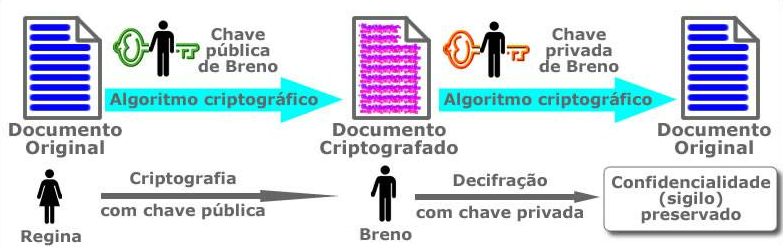
\includegraphics[width=.8\linewidth]{Figuras/Confidencialidade.png}
    \legend{Fonte: \cite{piropo07}}
\end{figure}

A autenticidade garante que quem enviou a mensagem foi o remetente. Quando se tem essa necessidade, deve-se criptografar a mensagem com a chave privada do remetente, enviar a mensagem criptografada para o destinatário, e ele, de posse da chave pública do remetente, poderá decriptografar a mensagem e assim obter a mensagem original.

O fato do destinatário ter conseguido decriptografar a mensagem com a chave pública do remetente comprova que a mensagem é realmente do remetente, mas não garante que o destinatário é o único que poderia decriptografar a mensagem, visto que qualquer pessoa pode possuir a chave pública do remetente, assim como demonstra a Figura \ref{fig:cripfocoauten}.

\begin{figure}[H]
    \centering
    \caption{Fluxo da mensagem criptografada quando o foco é autenticidade}
    \label{fig:cripfocoauten}
    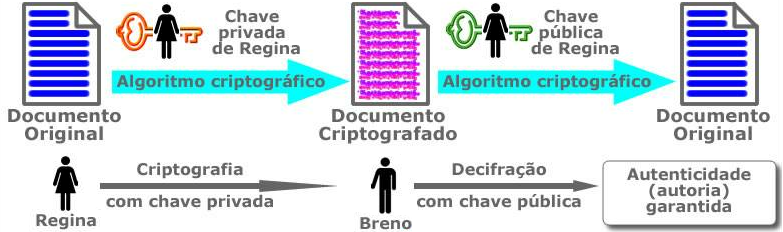
\includegraphics[width=.8\linewidth]{Figuras/Autencidade.png}
    \legend{Fonte: \cite{piropo07}}
\end{figure}

É possível também que se criptografe a mensagem com a chave privada do remetente, criptografar a mensagem já criptografada com a chave pública do destinatário, enviar a mensagem duplamente criptografada para o destinatário, e ele de posse da chave privada, poderá decriptografar a mensagem duplamente criptografada em uma mensagem criptografada e esta por sua vez será decriptografada com a chave pública do remetente e finalmente obter a mensagem original.

A combinação das duas criptografias, a com chave privada do remetente e com a chave publica do receptor, garante tanto que quem vai receber a mensagem é realmente o destinatário correto como garante que o remetente é quem ele diz ser \cite{stallings14} \cite{tanenbaum03}, assim como demonstra a Figura \ref{fig:cripfococonfieauten}.

\begin{figure}[H]
    \centering
    \caption{Fluxo da mensagem criptografada quando o foco é confidencialidade e autenticidade}
    \label{fig:cripfococonfieauten}
    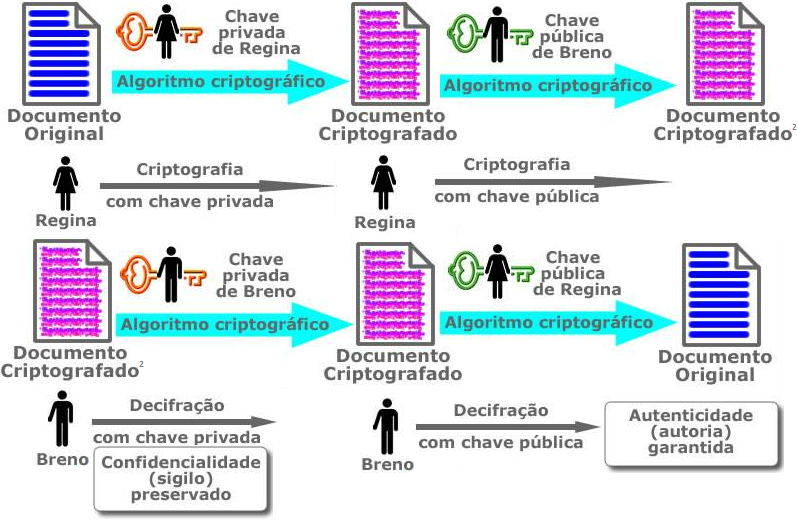
\includegraphics[width=.8\linewidth]{Figuras/ConfidEAuten.png}
    \legend{Fonte: \cite{piropo07}}
\end{figure}

\section{Cifra de blocos}
\label{sec:cifradeblocos}
A cifra de blocos manipula um bloco da mensagem clara como um todo e utiliza este para criar um bloco de mensagem cifrada de mesmo tamanho. É comum a utilização de um bloco com 64 ou 128 bits. Uma cifra de bloco pode ser usada para alcançar o mesmo efeito que uma cifra de fluxo. Cifras de fluxo trata de certo fluxo de dados singularmente, bit a bit ou byte a byte. São implementações clássicas das cifras de fluxo as cifras de \textit{Vigenère} auto chaveada e a cifra de Vernam e a mais utilizada atualmente é o RC4. A maioria das criptografias simétricas voltadas para ambientes de rede de computadores são implementadas com cifra de blocos e grande parte dos algoritmos de cifra de bloco simétrico usados na atualidade são baseados na cifra de blocos de \textit{Feistel}.

%A cifra de bloco trabalha com um bloco de dados da mensagem clara de n bits para produzir um bloco de mensagem cifrada de também de n bits. Se a cifra de bloco se utilizar de um n baixo então a cifra será equivalente a uma cifra de substituição simples. E se n for grande o suficiente e ainda assim for permitida a substituição reversível entre os blocos de mensagem cifrada e não cifrada, então a mensagem clara estaria tão camuflada que a criptoanálise se tornaria inviável.

\begin{figure}[H]
    \centering
    \caption{Cifra de bloco ideal}
    \label{fig:cifrablocoideal}
    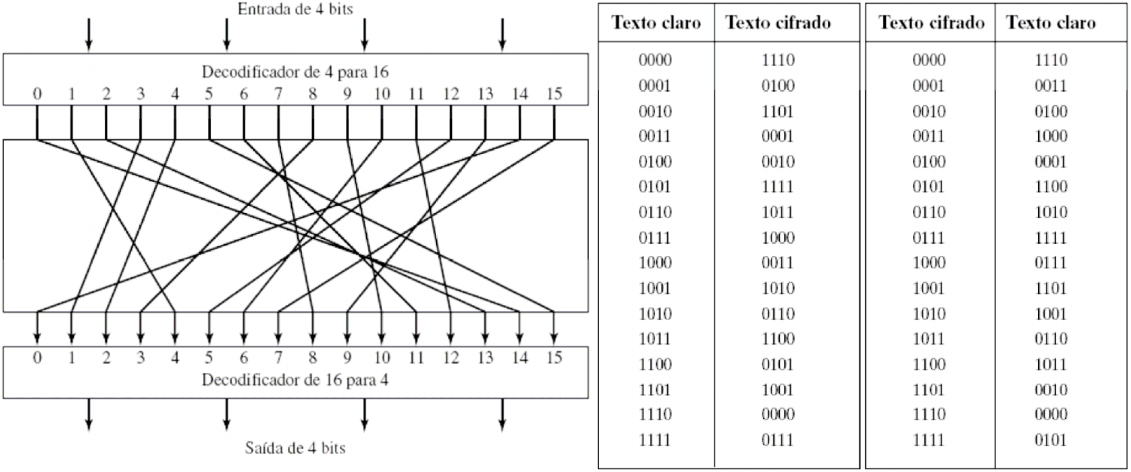
\includegraphics[width=.8\linewidth]{Figuras/CifraDeBloco.png}
    \legend{Fonte: \cite{stallings10}}
\end{figure}

Uma cifra de substituição reversível qualquer, \textit{Feistel} chamava esse cenário de cifra de bloco ideal, para um grande tamanho de bloco não é viável, do ponto de vista de desempenho e implementação, assim como demonstra a Figura \ref{fig:cifrablocoideal}. \textit{Feistel} propunha que era possível chegar mais próximo da cifra de bloco ideal. Era só utilizar uma cifra de produto, ou seja, a execução de duas ou mais cifras em sequência, tornando assim o produto final criptograficamente mais forte do que se poderia obter através de qualquer uma das cifras componentes do produto. A estrutura de \textit{Feistel} consiste em repetidas rodadas do mesmo procedimento. A cada vez que o procedimento se repete é realizada a substituição em metade dos dados da mensagem sendo processados, logo após se permuta as duas metades. A chave sendo utilizada é expandida de modo que uma chave diferente seja utilizada em cada iteração. Na prática \textit{Fiestel} propôs o uso de uma cifra que alternava entre substituições e permutações, o que na realidade é uma implementação prática do que \textit{Claude Shannon} já havia proposto como, cifra de produto que alterne confusão e difusão \cite{stallings14} \cite{tanenbaum03}.

\section{DES}
\label{sec:des}
Foi estabelecido pela IBM no final da década de 1960 um projeto de pesquisa sobre criptografia de computadores que trazia a sua frente \textit{Horst Feistel}. Com a conclusão do projeto em 1971 foi apresentado como resultado um algoritmo denominado LUCIFER, que foi comercializado ao \textit{Lloyd’s} localizado em Londres para ser utilizado em um sistema de caixa eletrônico que também havia sido desenvolvido pela IBM. LUCIFER é uma cifra de bloco de \textit{Feistel} que operava com blocos de 64 bits e se utilizava de uma palavra com tamanho de 128 bits.

Com o sucesso do LUCIFER a IBM mobilizou um novo projeto, dessa vez com o intuito de tornar o LUCIFER comercializável em grande escala, conseguindo coloca-lo em um único chip. Este projeto, que por sua vez era liderado por \textit{Walter Tuchman} e \textit{Carl Meyer}, contava com a ajuda tanto de consultores externos como orientação técnica da \acrfull{nsa}. O resultado deste novo projeto foi um LUCIFER mais refinado e mais resistente à criptoanálise, mas continha um tamanho de chave de 56 bits, para poder caber em um chip.

A \acrfull{nbs}, em 1973, solicitou propostas de uma cifra para ser padronizada a nível nacional. A IBM enviou o LUCIFER refinado, o que continha 56 bits, e por ser o melhor algoritmo proposto foi, em 1977, adotado como \acrfull{des}.

Com uma chave de 56 bits, existem ao todo 256 possíveis chaves, algo próximo de 7,2 x 1016 chaves. Aparentemente, um número tão grande de possibilidades é algo praticamente impossível de se descobrir se utilizando o método de força bruta. Por exemplo, uma única máquina processando uma criptografia \acrshort{des} por microssegundo levaria mais de mil anos para quebrar a cifra.

Por mais que para as máquinas de hoje, uma criptografia \acrshort{des} a cada microssegundo pareça irreal, pois a velocidade das máquinas de hoje já é bem superior as máquinas da década de 70, para aquela época não era algo tão simples. Mesmo assim, em 1977, \textit{Diffie} e \textit{Hellman} declararam que já existia tecnologia suficiente para se criar uma máquina que concentraria, de forma paralela, um milhão de dispositivos criptográficos, cada um com o poder de processamento da máquina citada no exemplo anterior. Isso reduziria o tempo de quebra da cifra para cerca de dez horas. Infelizmente, tal configuração na época custaria em torno de vinte milhões de dólares.

Finalmente, em 1998, vinte e um anos depois, o \acrshort{des} provou ser inseguro, quando a \acrfull{eff} anunciou que tinha quebrado uma cifra \acrshort{des} utilizando uma máquina “decifradora de DES” montada por menos de 250 mil dólares. Como se isso já não fosse suficiente para tornar o \acrshort{des} um algoritmo criptográfico ultrapassado, ainda existe a constante evolução do hardware, aumentando cada vez mais a velocidade de processamento e consequentemente possibilitando tanto que o método da força bruta seja mais viável, temporalmente falando, como também que sejam criados algoritmos de criptografia que se utilizem melhor desse novo poder de processamento.

Felizmente já existem várias alternativas para o \acrshort{des}, entre elas estão o \acrfull{aes} e o \acrfull{3des} \cite{stallings14} \cite{tanenbaum03}.

\section{3DES}
\label{sec:3des}
A criptografia múltipla é quando um algoritmo de criptografia é utilizado repetidas vezes. Primeiramente, a mensagem clara é criptografada utilizando um algoritmo de criptografia. A mensagem cifrada é então usada como entrada para um algoritmo de criptografia, podendo ser o mesmo utilizado anteriormente ou algum outro algoritmo, e esse processo pode ser repetir por indefinidas vezes.

O \acrfull{3des} é um exemplo de criptografia múltipla. Ele se utiliza do algoritmo \acrshort{des} três vezes, usando duas ou três chaves diferentes.

Em seu estado inicial a criptografia múltipla possui dois estágios, no caso do \acrshort{des} duplo, cada um se utilizando de uma chave diferente uma da outra, a criptografia E de uma mensagem M se utilizando de duas chaves \(K_1\) e \(K_2\) resultando em um texto criptografado C seria assim:

\[C = E(K_2, E(K_1, M))\]

Já a sua decriptografia D seria assim, aplicando as chaves inversamente:

\[M = D(K_1, D(K_2, C))\]

O \acrshort{des} triplo veio como uma alternativa clara para sanar o problema do \acrshort{des} simples, gerado pelo avanço computacional, uma vez que aumenta o custo do ataque da mensagem clara conhecida para 2112 (quando se utiliza de duas chaves) o que está além do possível, pelo menos, atualmente. Mas se utilizar de três estágios com três chaves diferentes exige um tamanho de chave de 168 bits (56 x 3), o que pode ser custoso.

Para diminuir o problema citado, \textit{Tuchman} propôs uma alternativa se utilizando somente de duas chaves:

\[C = E(K_1, D(K_2, E(K_1, M)))\]

A solução acima apresentada se tornou relativamente popular tendo sida adotada para uso nos padrões de gerenciamento de chaves ANS X9.17 e ISO 8732.

Atualmente contra o \acrshort{3des} não existem ataques criptoanalíticos práticos, visto que, o custo de uma pesquisa de chave por força bruta seria de uma complexidade de ordem \(2^{56} \times 2^{56} = 2^{112}\) (quando fossem utilizadas somente duas chaves) o que é equivalente a aproximadamente \(5 \times 10^{33}\).

Mesmo o \acrshort{3des} com duas chaves sendo de difícil ataque, ainda pode haver uma certa preocupação. Portanto pesquisadores creem que o melhor seria se utilizar do \acrshort{3des} com três chaves. Como já dito anteriormente o \acrshort{3des} com três chaves possui uma chave de tamanho efetivo de 168 bits, o que a torna mais segura em relação com o de duas chaves, e possui a seguinte forma \cite{stallings14}:

\[C = E(K_3, D(K_2, E(K_1, M))\]

\section{S-DES}
\label{sec:sdes}
O \acrfull{sdes}, desenvolvido pelo professor \textit{Edward Schaefer} da \textit{Santa Clara University} \cite{schaefer96}, é uma versão simplificada e voltada ao ensino do algoritmo \acrfull{des} do qual possui as mesmas propriedades e estrutura tendo como únicas divergências o tamanho reduzido dos parâmetros de entrada e o número reduzido de execuções da função \(f_K\). Enquanto o \acrshort{des} recebe como entrada blocos de 64 bits, usa 1 chave de 56 bits de onde se extraem 16 chaves de 48 bits (cada uma será utiliza em uma das 16 aplicações de \(f_K\)) e retorna como saída blocos de 64 bits o \acrshort{sdes} recebe como entrada 1 bloco de 8 bits, usa 1 chave de 10 bits de onde se extraem 2 chaves de 8 bits (cada uma será utilizada em uma das 2 aplicações de \(f_K\)) e retorna como saída 1 bloco de 8 bits. Essas reduções tornam o \acrshort{sdes} o melhor candidato para análise quando o objetivo é aprendizado. \cite{stallings10} \cite{stallings14}

A figura \ref{fig:sdesscheme} apresenta a estrutura geral do \acrshort{sdes}. Nela pode-se observar quais são as etapas que geram as chaves, quais etapas e ordem destas criptografam o \textit{plaintext} e quais etapas e ordem destas descriptografram o \textit{ciphertext}.

\begin{figure}[H]
    \centering
    \caption{Estrutura do \acrshort{sdes}}
    \label{fig:sdesscheme}
    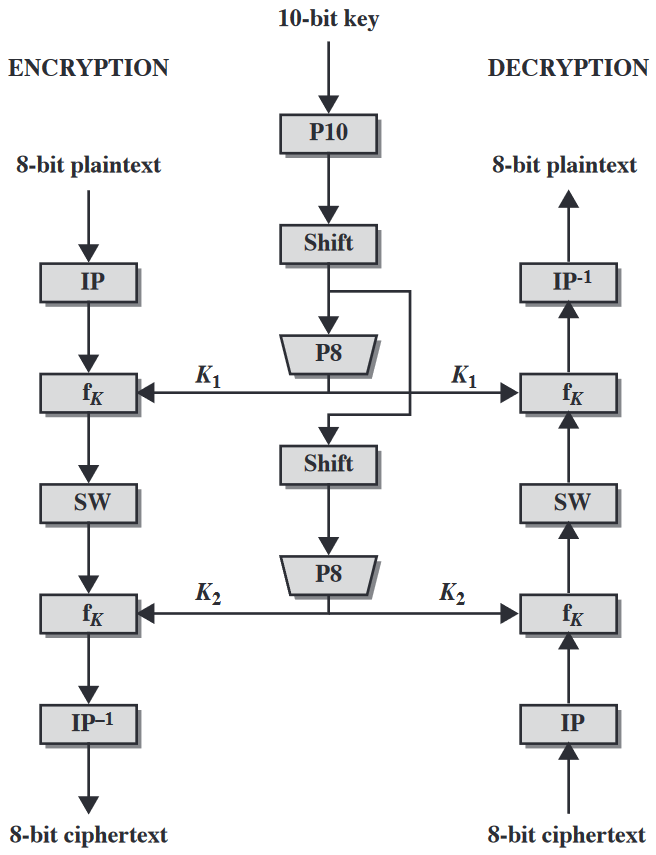
\includegraphics[width=.5\linewidth]{Figuras/SDESScheme.png}
    \legend{Fonte: "Figura G.1 do apêndice G" \cite{stallings10}}
\end{figure}

Pode-se expressar matematicamente o algoritmo de criptografia como uma composição de funções:

\[IP^{-1} \circ f_{K_2} \circ SW \circ f_{K_1} \circ IP\]

Ou de maneira mais direta:

\[ciphertext = IP^{-1}(f_{K_2}(SW(f_{K_1}(IP(plaintext)))))\]

Similarmente pode-se expressar o algoritmo de descriptografia:

\[IP^{-1} \circ f_{K_1} \circ SW \circ f_{K_2} \circ IP\]

Ou também:

\[plaintext = IP^{-1}(f_{K_1}(SW(f_{K_2}(IP(ciphertext)))))\]

\begin{figure}[H]
    \centering
    \caption{Geração das Chaves do \acrshort{sdes}}
    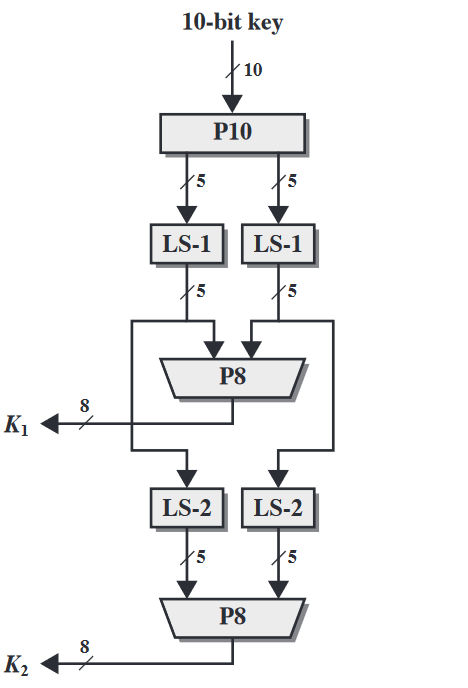
\includegraphics[width=.5\linewidth]{Figuras/SDESKeysGen.png}
    \legend{Fonte: "Figura G.2 do apêndice G" \cite{stallings10}}
\end{figure}

A geração das chaves pode ser expressada através das seguintes:

\[K_1 = P8(Shift_1(P10(key)))\]
\[K_2 = P8(Shift_2(Shift_1(P10(key))))\]

A figura \ref{fig:sdesdetail} demonstra de forma mais detalha o fluxo de execução de criptografia do \acrshort{sdes}. Nesta a função \(f_K\) é detalhada. Esta recebe por sua vez 3 parâmetros: \(L\), \(R\) e \(K\). \(L\) é a metade esquerda dos bits recebidos do passo anterior, \(R\) são os bits restantes, ou seja, a metade direita e \(K\) é a \textit{key} que deve ser utilizada. Sendo assim, temos:

\[f_K(L, R) = (L \oplus F(R, K), R)\]

A função \(F\) por sua vez não é tão diretamente explicita matematicamente mas seu fluxo também pode ser analisado na figura \ref{fig:sdesdetail}. \cite{stallings10}

A descrição detalhada completa do fluxo de execução do \acrshort{sdes} pode ser encontrada no simulador desenvolvido.

\begin{figure}[H]
    \centering
    \caption{Detalhamento da criptografia do \acrshort{sdes}}
    \label{fig:sdesdetail}
    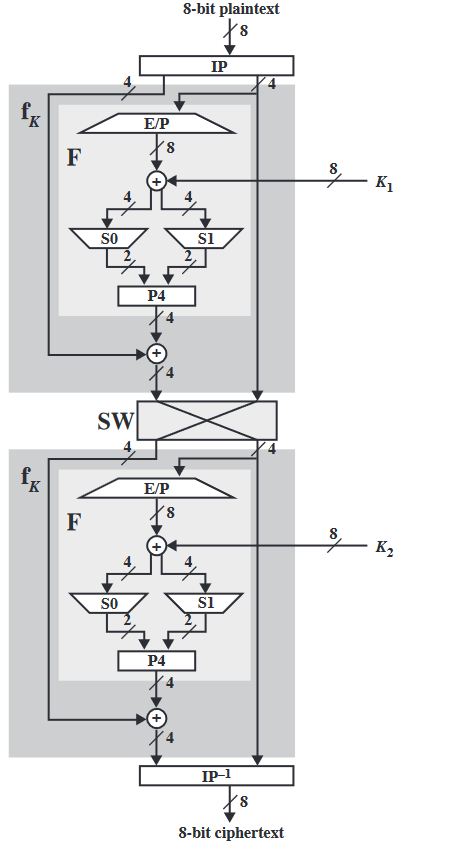
\includegraphics[width=.5\linewidth]{Figuras/SDESEncrypDetail.png}
    \legend{Fonte: "Figura G.3 do apêndice G" \cite{stallings10}}
\end{figure}

%Há também a Esteganografia que não faz parte de Criptologia, mesmo sendo estudada em situações bem similares e até pelos mesmos autores. Ao contrário da criptografia que modifica a informação com intuito de transformar seu estado original em algo indecifrável a Esteganografia estuda formas de como se pode camuflar uma informação dentro de outra. Temos também a Esteganálise que está para Esteganogr
